\documentclass[12pt]{beamer}
\usetheme{Boadilla}
\usepackage{tikz}
\usepackage{pgfplots}
\renewcommand{\arraystretch}{1.25}
\usetikzlibrary{trees}
\title[ECON2843]{Lecture 2}
\subtitle{Part 1 Descriptive Statics, Summary Measures, and Data Visualization}
\date{}
\usepackage{amsmath,amssymb,mathtools,wasysym}
\begin{document}
\begin{frame}
	\titlepage
\end{frame}
	\begin{frame}{Arithmetic Mean}
		\[
		\text{Arithmetic Mean} = \frac{1}{n} \sum_{i=1}^{n} X_i
		\]
		\begin{itemize}
			\item[$\blacktriangleright$] The arithmetic mean is the sum of all data points divided by the number of points.
			\item[$\blacktriangleright$] It is the most commonly used mean and represents a balance point of the data.
		\end{itemize}
		\textbf{Example:}
		\begin{itemize}
			\item[$\blacktriangleright$] For the data set \( \{3, 5, 7, 9\} \), the arithmetic mean is \( \frac{3 + 5 + 7 + 9}{4} = 6 \).
		\end{itemize}
	\end{frame}
	\begin{frame}{Geometric Mean}
		\[
		\text{Geometric Mean} = \left( \prod_{i=1}^{n} X_i \right)^{\frac{1}{n}}
		\]
		\begin{itemize}
			\item[$\blacktriangleright$] The geometric mean is the nth root of the product of all data points.
			\item[$\blacktriangleright$] It is useful for data that are multiplicative or vary exponentially.
		\end{itemize}
		\textbf{Example:}
		\begin{itemize}
			\item[$\blacktriangleright$] For the data set \( \{1, 3, 9\} \), the geometric mean is \( (1 \times 3 \times 9)^{\frac{1}{3}} = 3 \).
		\end{itemize}
	\end{frame}
	\begin{frame}{Harmonic Mean}
		\[
		\text{Harmonic Mean} = \frac{n}{\sum_{i=1}^{n} \frac{1}{X_i}}
		\]
		\begin{itemize}
			\item[$\blacktriangleright$] The harmonic mean is the reciprocal of the arithmetic mean of the reciprocals.
			\item[$\blacktriangleright$] It is useful for rates and ratios, such as speed or density.
		\end{itemize}
		\textbf{Example:}
		\begin{itemize}
			\item[$\blacktriangleright$] For the data set \( \{2, 3, 4\} \), the harmonic mean is \( \frac{3}{\frac{1}{2} + \frac{1}{3} + \frac{1}{4}} \approx 2.77 \).
		\end{itemize}
	\end{frame}
\begin{frame}{Harmonic Mean}
			The harmonic mean can be used to calculate the average speed when the distances are the same but the speeds differ. For example, if for a certain journey, the speed is 60 mph for the first half and 30 mph for the second half (with both distances being equal), the average speed is the harmonic mean of the two speeds, which is 40 mph.\medskip\\
			Assume the distance to be $a$, then the average speed is:
			$$\frac{\text{the distance}}{\text{the time spent}}=\frac{a}{\frac{0.5a}{30}+\frac{0.5a}{60}}=\frac{2}{\frac{1}{30}+\frac{1}{60}}=40$$
	\end{frame}
\begin{frame}{Variance}
	\begin{itemize}
		\item[$\blacktriangleright$]What we just calculated is known as the {\bf variance},which measures the spread or variability of a given distribution of data.
		\item[$\blacktriangleright$]Population variance:$$\sigma^2=\frac{1}{N}\sum_{i=1}^N(X_i-\mu)^2$$
		\item[$\blacktriangleright$]Sample variance:
		$$s^2=\frac{1}{n-1}\sum_{i=1}^n(X_i-\bar{X})^2$$
	\end{itemize}
\end{frame}
\begin{frame}{Why Sample Variance has $n-1$ on denominator?}
	\text{Recall the terms:}
	\begin{align*}
		& \mu = \text{population mean} \\
		& \sigma^2 = \text{population variance} \\
		& \bar{X} = \text{sample mean} \\
		& s^2 = \text{sample variance} \\
		& X_1, X_2, \cdots, X_n = \text{sample values}
	\end{align*}
\end{frame}
\begin{frame}{Why Sample Variance has $n-1$ on denominator?}
Let's start from this...\medskip\\
Flip a coin: if it lands heads up, you win $\$1$; if it lands tails up, you win $\$0$. Flip the coin ten times, how much do you think you can win?\medskip\\
What about if you flip it 100 or 1000 times? Do you think it will converge to a certain value as the number of flips increases?
\end{frame}
\begin{frame}{Law of Large Numbers}

{\bf Law of large numbers}:\medskip\\
If you repeat an experiment independently a large number of times and average the result, what you obtain should be close to the expected value.

In other words, if you take an infinite number of samples, the mean of the sample statistics will increasingly approach the population parameter.\medskip\\
\href{https://www.math.ucdavis.edu/~tracy/courses/math135A/UsefullCourseMaterial/lawLargeNo.pdf}{\color{blue}\underline{Link to proof if you are interested}}
\end{frame}
\begin{frame}{Why Sample Variance has $n-1$ on denominator?}
From the Law of large numbers we know: If we sample infinitely many times and calculate the {\color{red}average} of {\color{blue}mean} and {\color{blue}variance} we get:
	\[\mathbb E[\bar{X}]=\mu\]
	Then what about
	$$\mathbb E[\sum_{i=1}^n (X_i - \bar{X})^2]$$
	
	Note: $\mathbb E[\cdot]$ is a sign that denotes mathematical expectations.
\end{frame}
\begin{frame}
	\text{Recall the population variance formula:}
	$$\sigma^2=\frac{1}{N}\sum_{i=1}^N(X_i-\mu)^2$$
	\text{Sample variance:}
	\[s^2 = \frac{1}{n-1} \sum_{i=1}^n (X_i - \bar{X})^2\]
	\text{Rewrite $\mathbb E[\sum_{i=1}^n (X_i - \bar{X})^2]$ as:}
	\[\mathbb E[\sum_{i=1}^n (X_i - \mu + \mu - \bar{X})^2]\]
\end{frame}
\begin{frame}
	\text{Expand the squared term:}
	\[\mathbb E[\sum_{i=1}^n ((X_i - \mu)^2 + 2(X_i - \mu)(\mu - \bar{X}) + (\mu - \bar{X})^2)]\]
	
	\text{Simplify:}
	\[\mathbb E[\sum_{i=1}^n (X_i - \mu)^2] + \mathbb E[\sum_{i=1}^n 2(X_i - \mu)(\mu - \bar{X})] + \mathbb E[\sum_{i=1}^n (\mu - \bar{X})^2]\]
\end{frame}
\begin{frame}
	\text{The middle term equals zero because} $\mathbb E[\bar{X}] = \mu, \text{ so:}$
	\[\mathbb E[\sum_{i=1}^n (X_i - \mu)^2] + \mathbb E[n(\mu - \bar{X})^2]\]
	which is
		\[\mathbb E[\sum_{i=1}^n (X_i - \mu)^2] + n\mathbb E[(\mu - \bar{X})^2]\]
\text{We know that} $\mathbb E[\sum_{i=1}^n (X_i - \mu)^2] = n\sigma^2 \text{ and } \mathbb E[(\mu - \bar{X})^2] = \frac{\sigma^2}{n}, \text{ so:}$
	\[n\sigma^2 + n(\frac{\sigma^2}{n}) = n\sigma^2 + \sigma^2\]
\end{frame}
\begin{frame}	
	\text{Therefore:}
	\[\mathbb E[\sum_{i=1}^n (X_i - \bar{X})^2] = (n-1)\sigma^2\]
	
	\text{If we use $n$ in the denominator:}
	\[\mathbb E[\frac{1}{n}\sum_{i=1}^n (X_i - \bar{X})^2] = \frac{n-1}{n}\sigma^2\]
	
	This is biased because it's less than the true population variance $\sigma^2$.\medskip\\
	\text{But if we use $(n-1)$ in the denominator:}
	\[\mathbb E[\frac{1}{n-1}\sum_{i=1}^n (x_i - \bar{x})^2] = \sigma^2\]
	
	\text{This gives us an unbiased estimator of the population variance.}
\end{frame}
\begin{frame}{Standard Deviation}
\begin{itemize}
	\item[$\blacktriangleright$]Since we squared the observations when calculating the variance, the units for variance is the "original units" squared.
	\item[$\blacktriangleright$] The standard deviation is defined as the square-root of the variance.
	\item[$\blacktriangleright$] Conveys same information as variance, but is now in the "original units" of measure.
\end{itemize}
\end{frame}
\begin{frame}{Standard Deviation}
	\begin{itemize}
		\item[$\blacktriangleright$]Population standard deviation:
		$$\sigma=\sqrt{\frac{1}{N}\sum_{i=1}^N(X_i-\mu)^2}$$
		\item[$\blacktriangleright$]Sample standard deviation:
		$$s=\sqrt{\frac{1}{n-1}\sum_{i=1}^n(X_i-\bar{X})^2}$$
	\end{itemize}
\end{frame}
\begin{frame}{Application in Finance}
\begin{itemize}
		\item[$\blacktriangleright$] Understanding variability is very important in finance.
		\item[$\blacktriangleright$] Variance (or standard deviation) of an investment can be used as a measure of risk, e.g., on profits/return.
		\item[$\blacktriangleright$] Larger variance implies larger risk.
		\item[$\blacktriangleright$] Usually, the higher the expected rate of return, the higher the risk.
\end{itemize}
\end{frame}
\begin{frame}{Walmart}
	\centering
	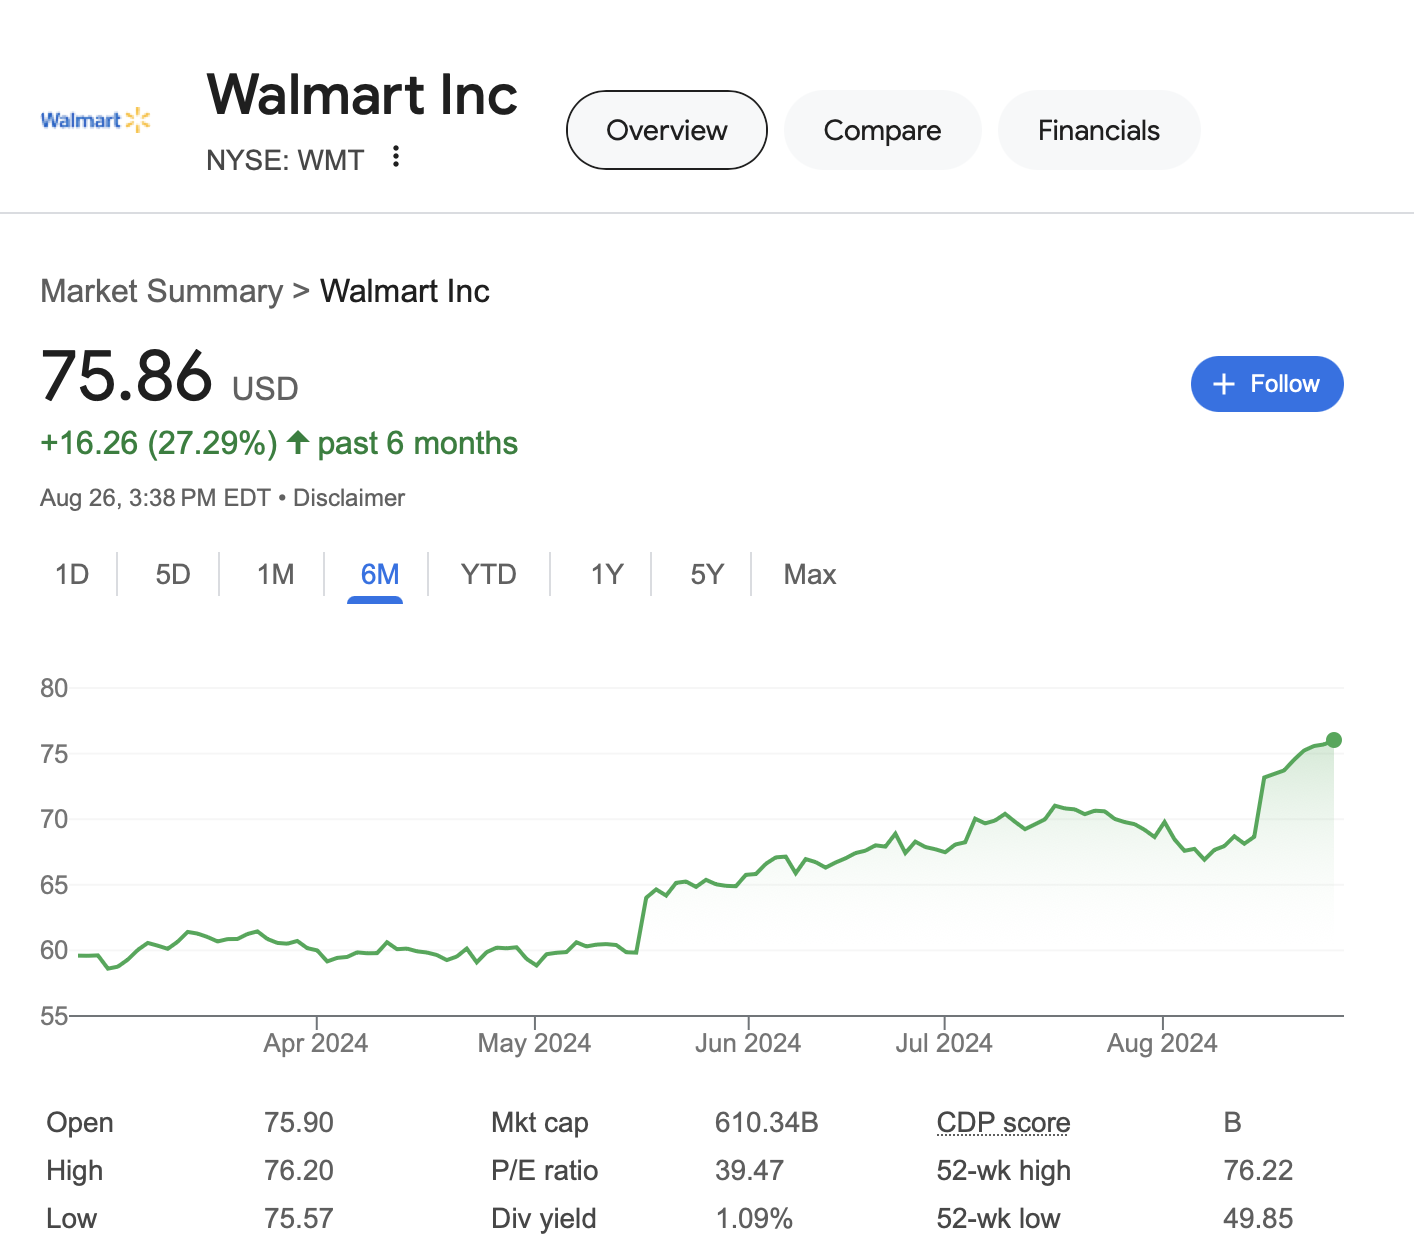
\includegraphics[width=9cm]{wmt.png}
\end{frame}
\begin{frame}{NVIDIA}
	\centering
	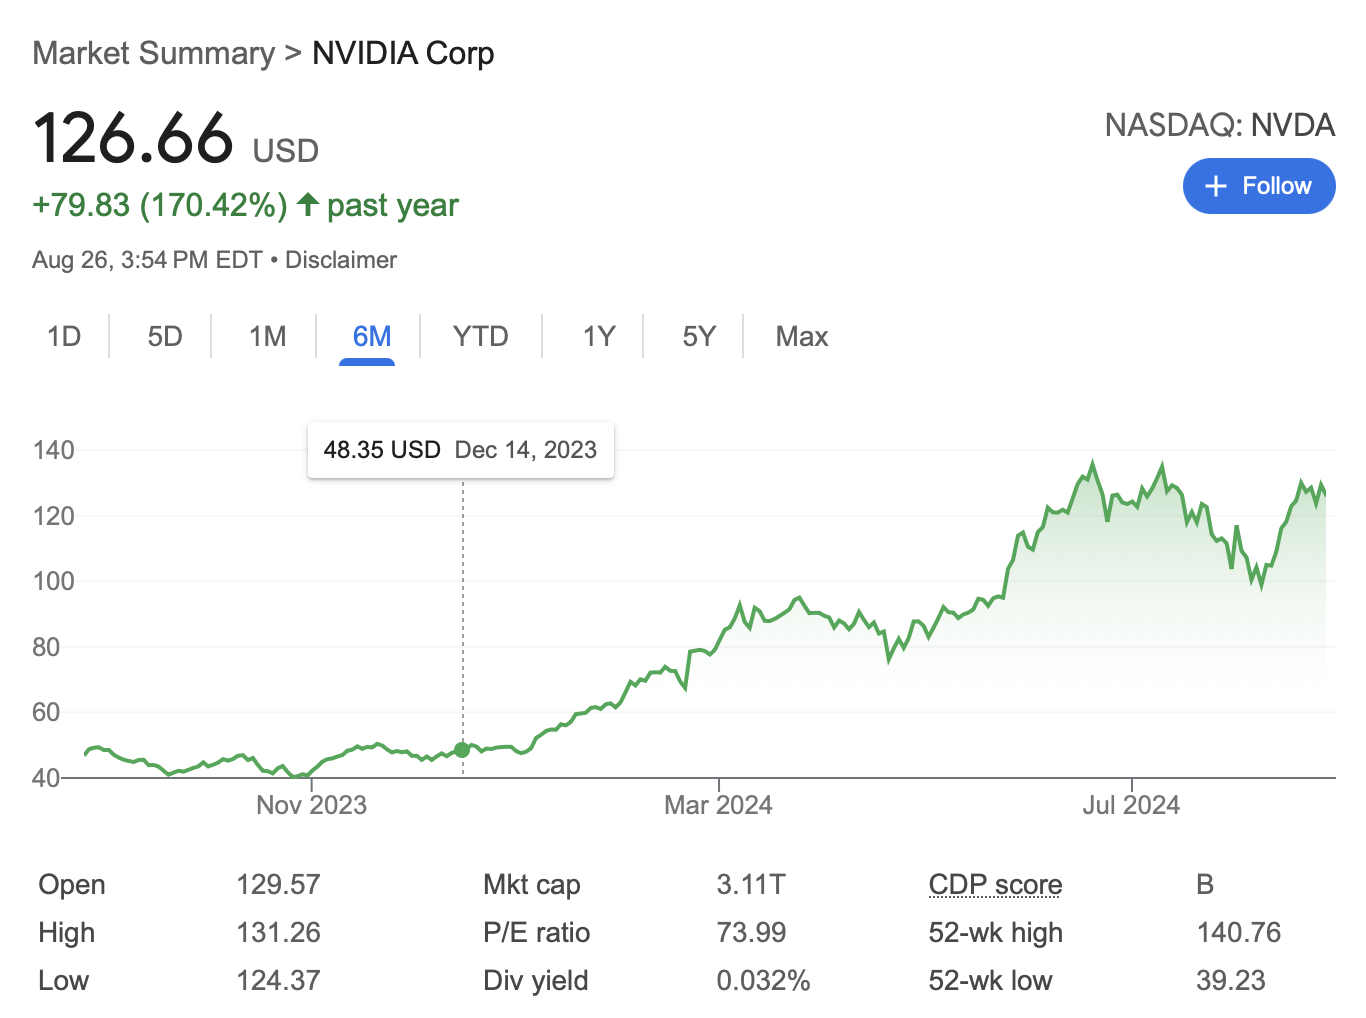
\includegraphics[width=9cm]{nvda.png}
\end{frame}
\begin{frame}{Bitcoin}
	\centering
	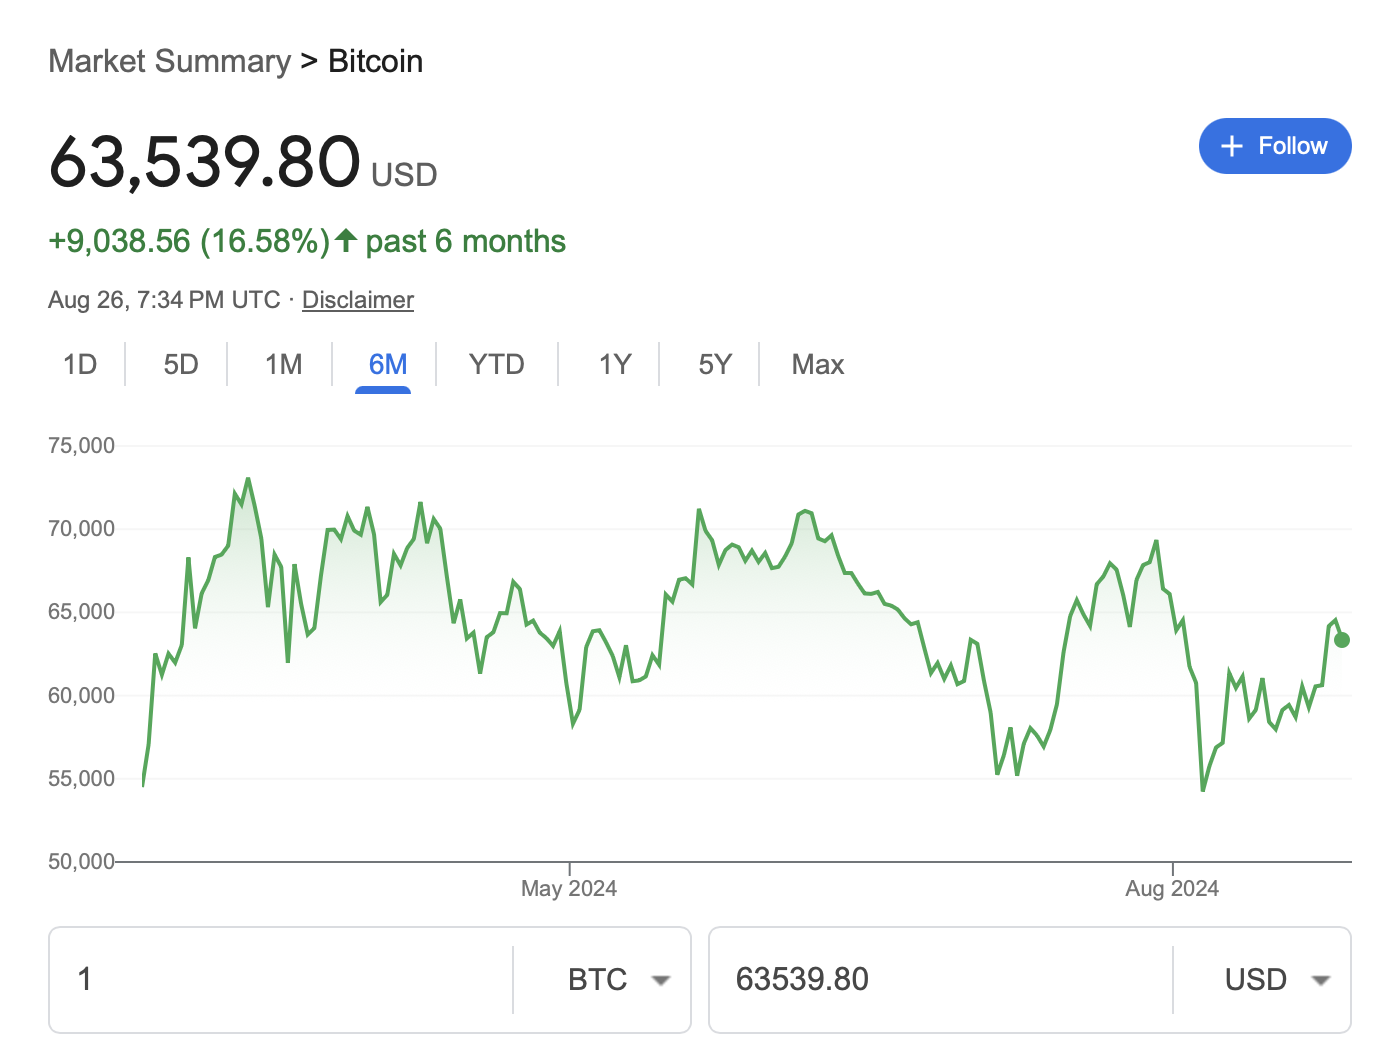
\includegraphics[width=9cm]{btc.png}
\end{frame}
\begin{frame}{Application in Finance}
	Rates of returns for two stocks $X$ and $Y$.
		\vspace{0.5cm}
		
		\begin{center}
			\begin{tabular}{|c|c|c|c|c|c|c|c|c|c|c|}
				\hline
				$X$ & 8.3 &-6.2&20.9 &-2.7 &33.6&42.9&24.4&5.2&3.1&30.5\\
				\hline
				$Y$ & 12.1 &-2.8& 6.4& 12.2&27.8&25.3&18.2&10.7&-1.3&11.4\\
				\hline
			\end{tabular}
		\end{center}
		\vspace{0.5cm}
$\bar{X}=16\%$ and $s_X^2=280.34\%^2$.

$\bar{Y}=12\%$ and $s_Y^2=99.37\%^2$.
\end{frame}
\begin{frame}{Application in Finance: Sharpe Ratio}
	\begin{itemize}
		\item[$\blacktriangleright$] It is a financial metric used to evaluate the risk-adjusted return of an investment or portfolio.
		\item[$\blacktriangleright$] The ratio helps investors understand how much excess return they are receiving for the extra volatility they endure for holding a riskier asset.
	\end{itemize}
\end{frame}
\begin{frame}{Sharpe Ratio}
	$$\text{Sharpe Ratio}=\frac{R_p-R_f}{\sigma_p}$$
	\begin{itemize}
		\item[$\blacktriangleright$] $R_p$: Return of a portfolio (portfolio here means combination of financial assets).
		\item[$\blacktriangleright$] $R_f$: Risk-free rate (typically the return of a government bond).
		\item[$\blacktriangleright$] $\sigma_p$: Standard deviation of the portfolio’s excess return (a measure of risk).
	\end{itemize}
\end{frame}
\begin{frame}{Sharpe Ratio}
	\begin{itemize}
		\item[$\blacktriangleright$] High Sharpe Ratio: Indicates that the investment is providing a higher return for the risk taken. It is generally seen as a sign of good investment performance.
		\item[$\blacktriangleright$] Low or Negative Sharpe Ratio: Indicates that the returns are not sufficient to justify the risk taken, or the investment is underperforming relative to a risk-free investment.
	\end{itemize}
\end{frame}
\begin{frame}{Sharpe Ratio}
	Rates of returns for two stocks $X$ and $Y$, assume a risk-free rate (CDs or bond rate) of 3\%.
	
	\begin{center}
		\begin{tabular}{|c|c|c|c|c|c|c|c|c|c|c|}
			\hline
			$X$ & 8.3 &-6.2&20.9 &-2.7 &33.6&42.9&24.4&5.2&3.1&30.5\\
			\hline
			$Y$ & 12.1 &-2.8& 6.4& 12.2&27.8&25.3&18.2&10.7&-1.3&11.4\\
			\hline
		\end{tabular}
\end{center}
\begin{center}
		\begin{tabular}{|c|c|c|c|c|c|c|c|c|c|c|}
			\hline
			$X-R_f$ & 5.3 &-9.2&17.9 &-5.7 &30.6&39.9&21.4&2.2&0.1&27.5\\
			\hline
			$Y-R_f$ & 9.1 &-5.8& 3.4& 9.2&24.8&22.3&15.2&7.7&-4.3&8.4\\
			\hline
		\end{tabular}
	\end{center}
	$\bar{X}-R_f=13\%$ and $s_{X-R_f}^2=280.34\%^2$.
	
	$\bar{Y}-R_f=9\%$ and $s_{Y-R_f}^2=99.37\%^2$.\medskip\\
	
	Question: Why $s^2$ remains the same?
\end{frame}
\begin{frame}{Sharpe Ratio}
The standard deviation is
	$s_{X-R_f}=16.74\%$ and $s_{Y-R_f}=9.97\%$.\medskip\\
	
So we have the Sharpe Ratios:
\begin{itemize}
	\item[$\blacktriangleright$] For stock $X$:
	$$\frac{\bar{X}-R_f}{s_{X-R_f}}=\frac{13\%}{16.74\%}=0.78$$
	\item[$\blacktriangleright$] For stock $Y$:
	$$\frac{\bar{Y}-R_f}{s_{Y-R_f}}=\frac{9}{9.97}=0.90$$
\end{itemize}
\end{frame}
\begin{frame}{Coefficient of Variation}
The {\bf coefficient of variation} is a measure of variability defined as the standard deviation divided by the mean.
	\begin{itemize}
		\item[$\blacktriangleright$] Population:
		$$CV=\frac{\sigma}{\mu}$$
		\item[$\blacktriangleright$] Sample:
		$$cv=\frac{s}{\bar{X}}$$
		\item[$\blacktriangleright$] Takes into account scale or magnitude of your data.
	\end{itemize}
\end{frame}
\begin{frame}{Covariance}
	
	{\bf Covariance} is a measure of the linear relationship between two variables and describes how they move in relates to one another.
	\begin{itemize}
		\item[$\blacktriangleright$] Why might this be important?
		\item[$\blacktriangleright$] Example: We have two stocks, $X$ and $Y$. Let's suppose that $X$ moves exactly with the market,whereas $Y$ moves opposite to the market.
	\end{itemize}
\end{frame}
\begin{frame}{Covariance}
	
	\begin{itemize}
		\item[$\blacktriangleright$] Scenario 1: You invest all your money in stock $X$. The market does really well. Stock $X$ pays off $\$1000$.
		\item[$\blacktriangleright$] Scenario 2: You invest all your money in stock $Y$. The market crashes. Stock $Y$ pays off $\$1000$.
		\item[$\blacktriangleright$] Covariance is very important in forming a portfolio.
	\end{itemize}
\end{frame}
\begin{frame}{Covariance}
	
	\begin{itemize}
		\item[$\blacktriangleright$] Population covariance:
		$$\sigma_{XY}=\frac{1}{N}\sum_{i=1}^N(X_i-\mu_X)(Y_i-\mu_Y)$$
		\item[$\blacktriangleright$] Sample covariance:
		$$s_{XY}=\frac{1}{n-1}\sum_{i=1}^n(X_i-\bar{X})(Y_i-\bar{Y})$$
	\end{itemize}
\end{frame}
\begin{frame}{Covariance}
	
	Another example.
	\begin{itemize}
		\item[$\blacktriangleright$] Let's say we're interested in how closely fathers' heights are related to sons' heights.
		\item[$\blacktriangleright$] The logical thing to do is to calculate the covariance of fathers' and sons' heights, right?
		\item[$\blacktriangleright$] Suppose we do that and find the covariance to be $20cm^2$.
	\end{itemize}
\end{frame}
\begin{frame}{Covariance}
	\begin{itemize}
		\item[$\blacktriangleright$] What if we're also interested in the relationship between the number of years of education of mothers and daughters?
		\item[$\blacktriangleright$] Once again, suppose we calculate the covariance of mothers' and daughters' years of education, and find it to be 3.5 years$^2$.
		\item[$\blacktriangleright$] Now, are fathers' and sons' heights more closely related to each other than mothers' and daughters' years of education?
	\end{itemize}
\end{frame}
\begin{frame}{Correlation Coefficient}
	\begin{itemize}
		\item[$\blacktriangleright$] {\bf Correlation} is also a measure of the linear relationship between two variables.
		\item[$\blacktriangleright$] Population correlation coefficient:
		$$\rho_{XY}=\frac{\sigma_{XY}}{\sigma_X\sigma_Y}$$
		\item[$\blacktriangleright$] Sample correlation coefficient:
		$$r_{XY}=\frac{s_{XY}}{s_Xs_Y}$$
	\end{itemize}
\end{frame}
\begin{frame}{Correlation Coefficient}
	\begin{itemize}
		\item[$\blacktriangleright$] A correlation coefficient standardizes the covariance of two variables such that its value will lie between $-1$ and 1 (inclusive).
		\item[$\blacktriangleright$] The interpretation is more intuitive than covariance,and direct comparisons between variables in different units of measure can be conducted.
		\item[$\blacktriangleright$] So, we could compare the correlation between fathers' and sons' heights to the correlation between mothers' and daughters' years of education.
	\end{itemize}
\end{frame}
\begin{frame}{Scatter Plots}
If $0<r_{XY}\le1$ then we have a positive linear relationship, with the strength dependent on how close $r_{XY}$ is to 1:
\centering
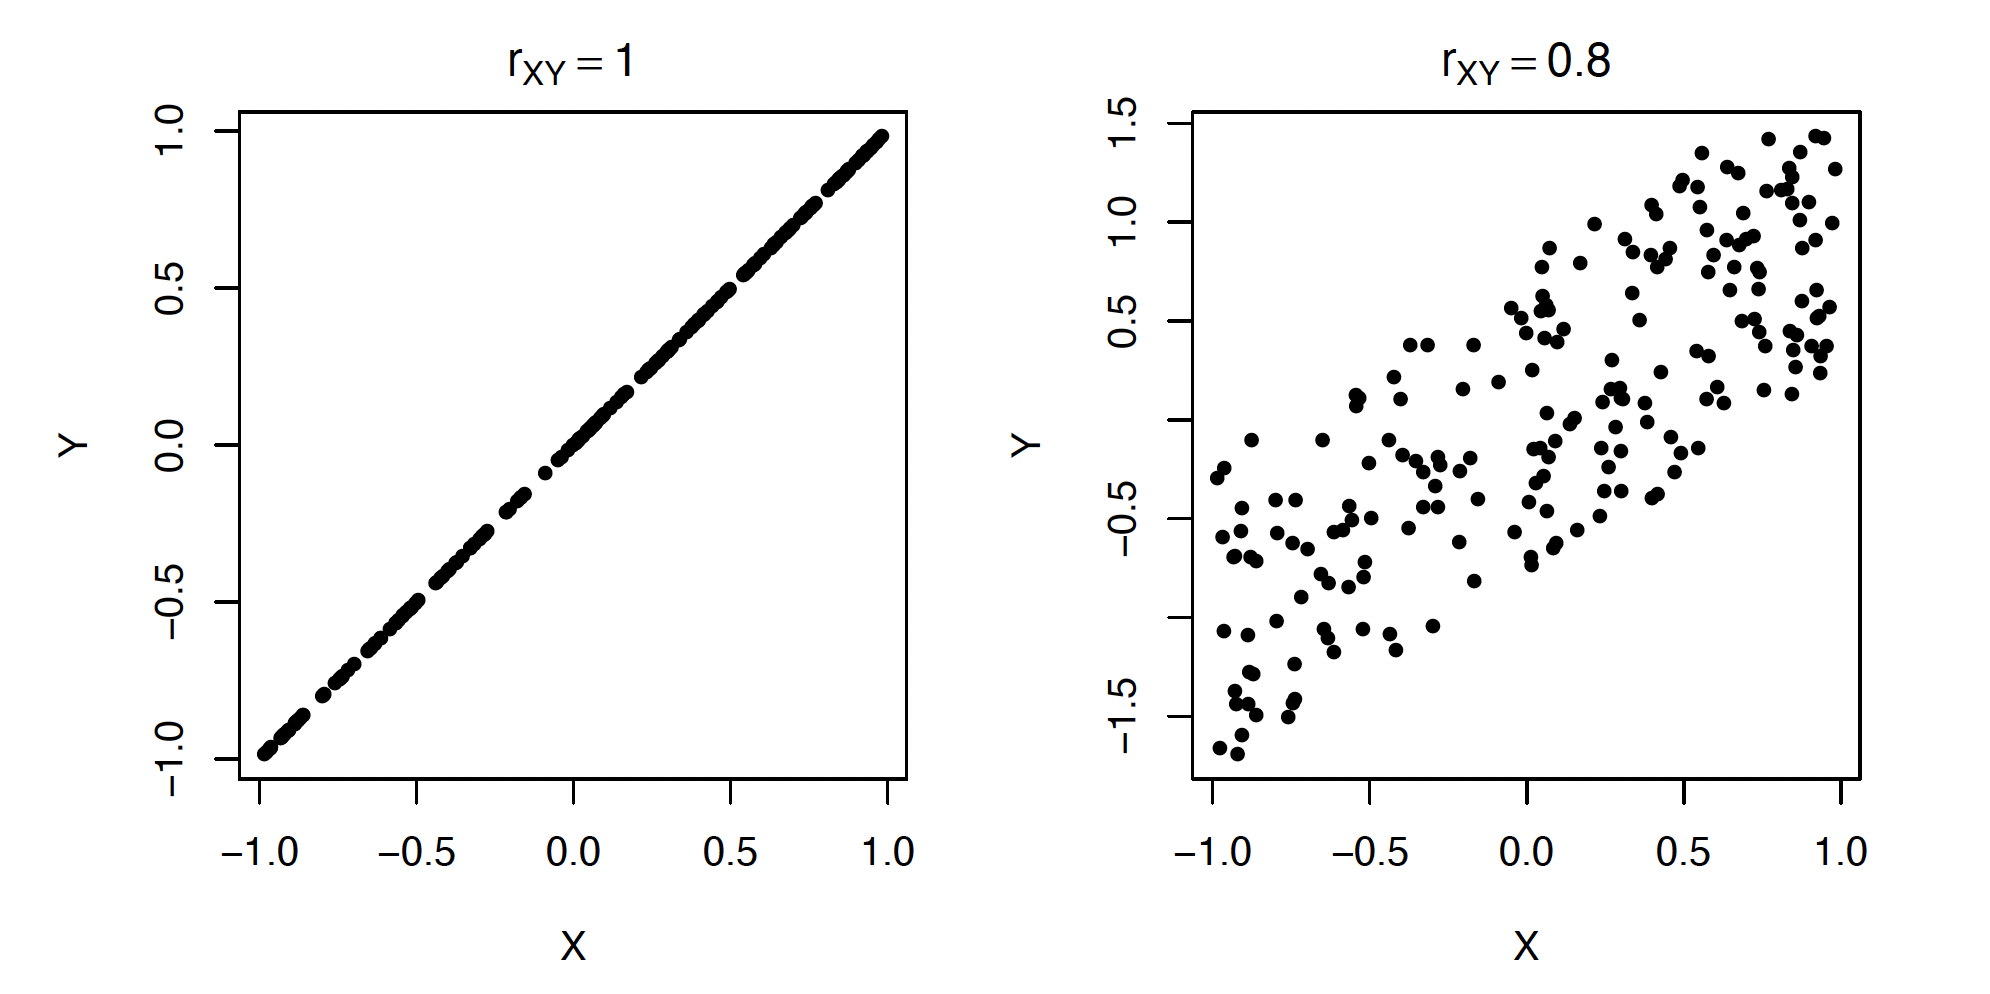
\includegraphics[width=12cm]{scatter.png}
\end{frame}
\begin{frame}{Scatter Plots}
	If $-1\le r_{XY}<0$ then we have a negative linear relationship, with the strength dependent on how close $r_{XY}$ is to $-1$:
	\centering
	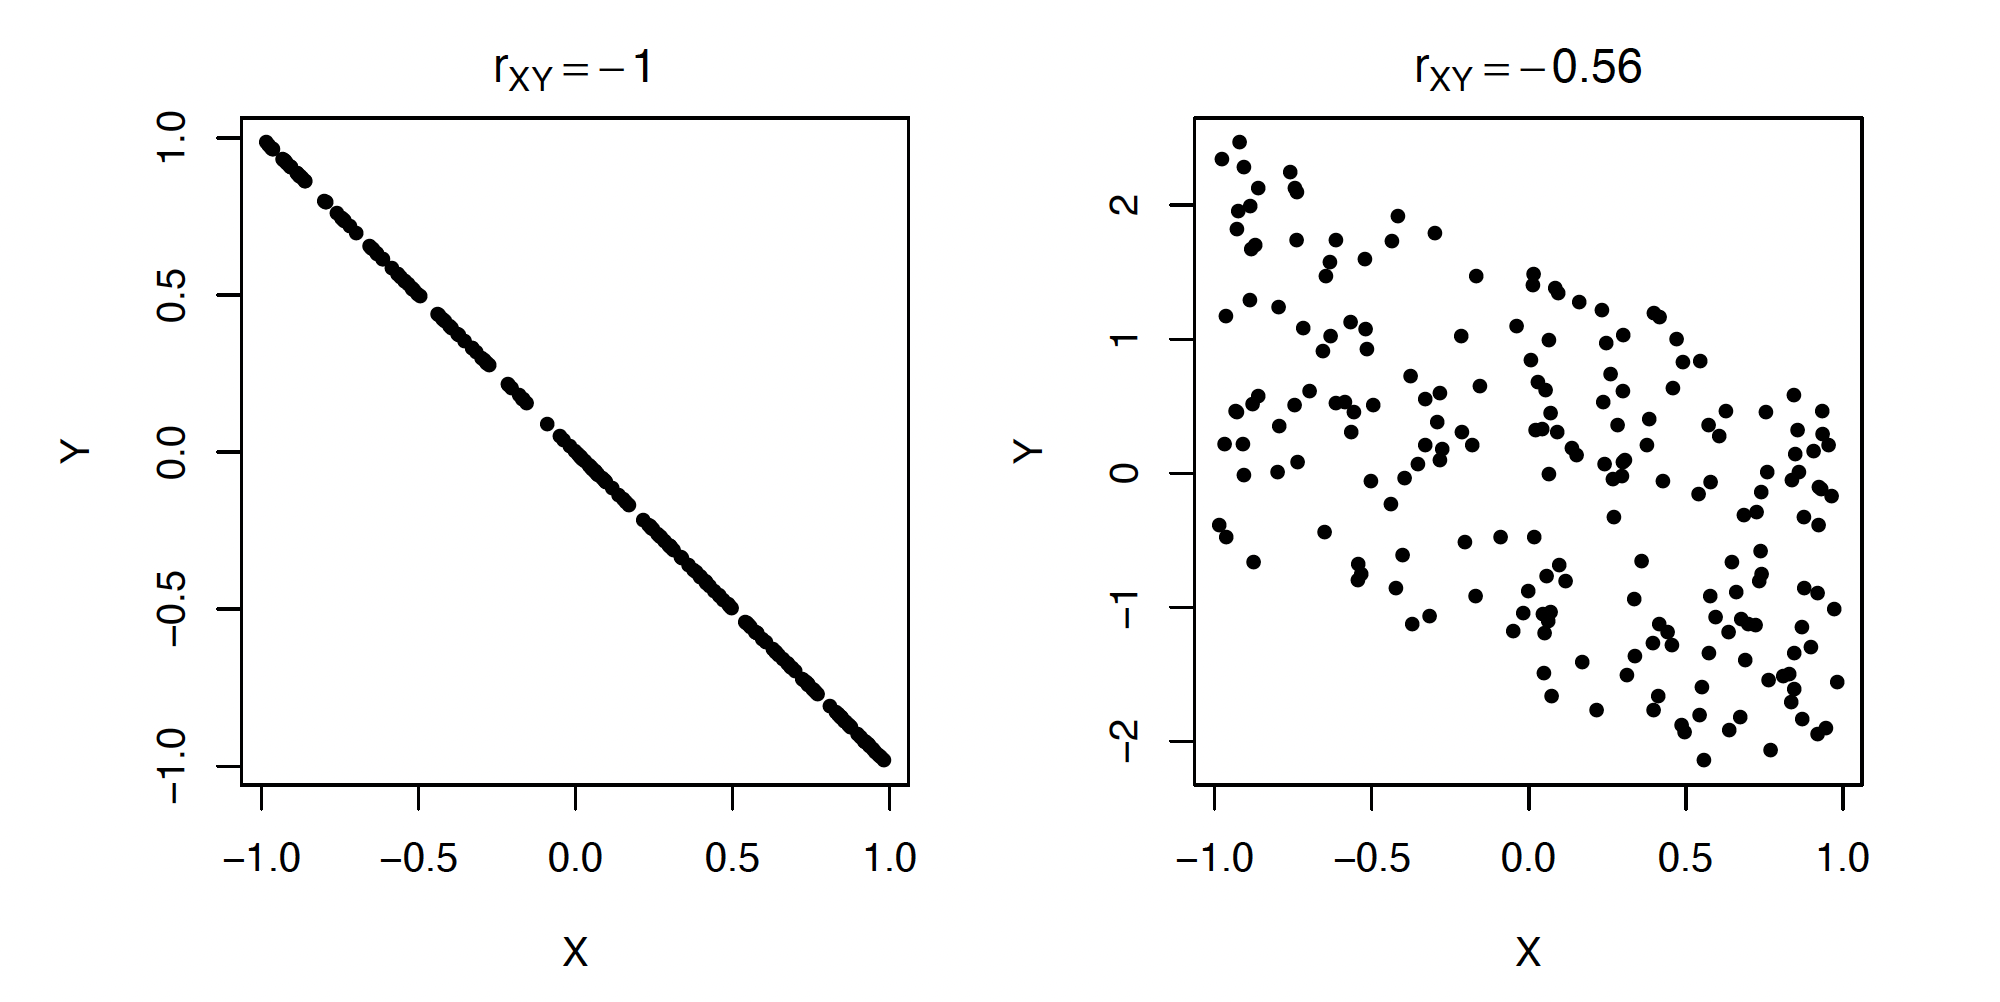
\includegraphics[width=12cm]{scatter2.png}
\end{frame}
\begin{frame}{Scatter Plots}
	If $r_{XY}\approx0$ then we have no linear relationship:
	\centering
	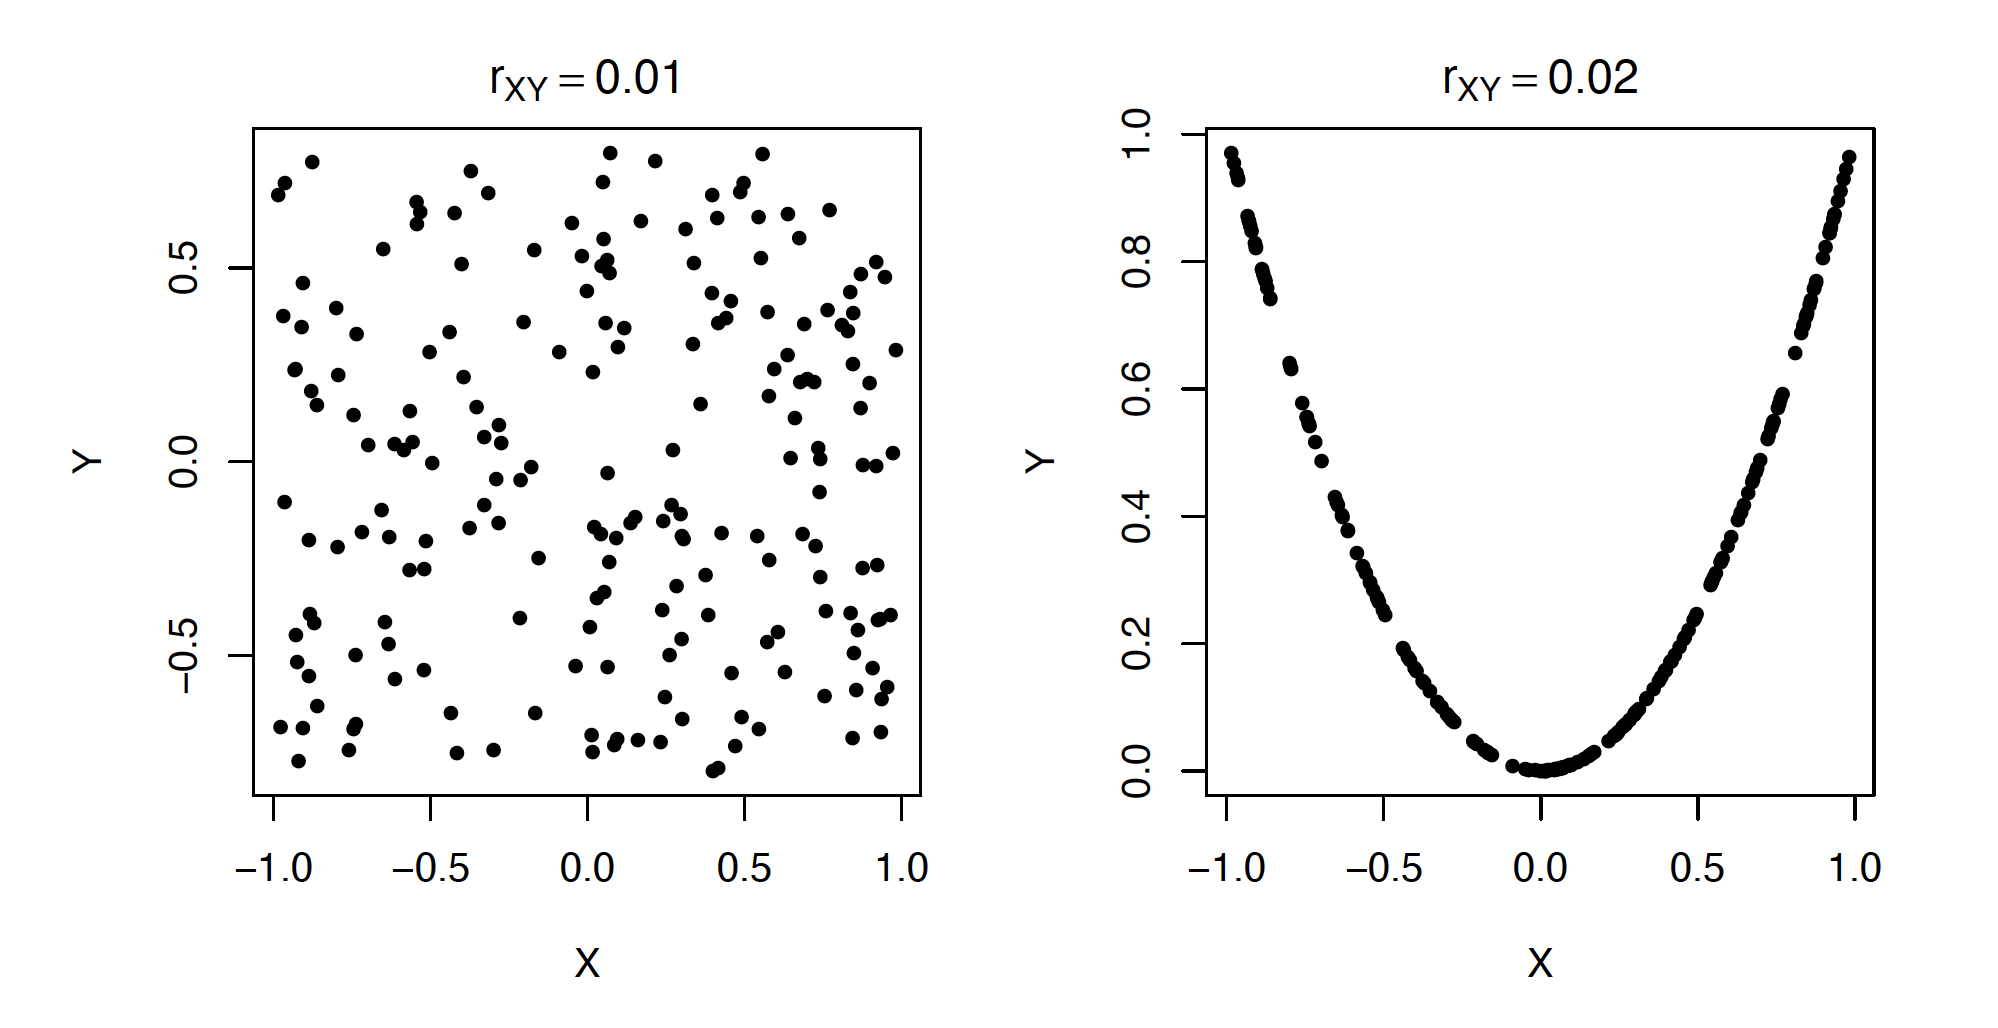
\includegraphics[width=12cm]{scatter3.png}
\end{frame}
\begin{frame}{Correlation and Causation}
	
{\bf\color{red}Note that correlation does not imply causation.}\medskip\\
Examples of variables that could be correlated but no causal relationship:
\begin{itemize}
	\item[$\blacktriangleright$] Number of ice cream sales and the rate of drowning deaths.
\end{itemize}
\end{frame}
\end{document}
